Veamos las conclusiones que extraemos de nuestro estudio tras todo este proceso:

\begin{enumerate}
\item La aplicación parece tener un mayor uso durante el fin de semana y el viernes.
\item Se producen más avistamientos de pokemon durante la noche (no sólo de pokemon de tipo fantasma como suponíamos en un inicio).
\item Hay muchos atributos en este dataset que parecen no aportar información. El creador del dataset además ha añadido más atributos de los que puede obtener directamente de la aplicación, esta información adicional tampoco parece ser de utilidad.
\item No hemos de centrarnos sólo en resolver el principal problema que plantea un dataset, en este caso la clasificación. Un dataset puede tener más utilidad que la de resolver el problema que plantea, por ejemplo en nuestro caso hemos aprovechado el extendido uso de esta aplicación para obtener un mapa de temperaturas para una semana de agosto.
\item Hay ocasiones en que la descripción que nos dan de un dataset puede no ser la correcta y tendremos que tratar de averiguar si los datos que se nos proporcionan son realmente lo que el creador del dataset dice que son.
\item A la luz de los resultados de la clasificación y de la extracción de reglas de asociación parece que los avistamiento de pokemon, al menos en las cinco especies que hemos escogido (aunque ya vimos que también se daba para el conjunto entero), tiene una componente aleatoria.
\end{enumerate}

En cuanto a esta última observación vamos a ver una serie de gráficas que parecen poner de manifiesto la aleatoriedad de los avistamientos:\\

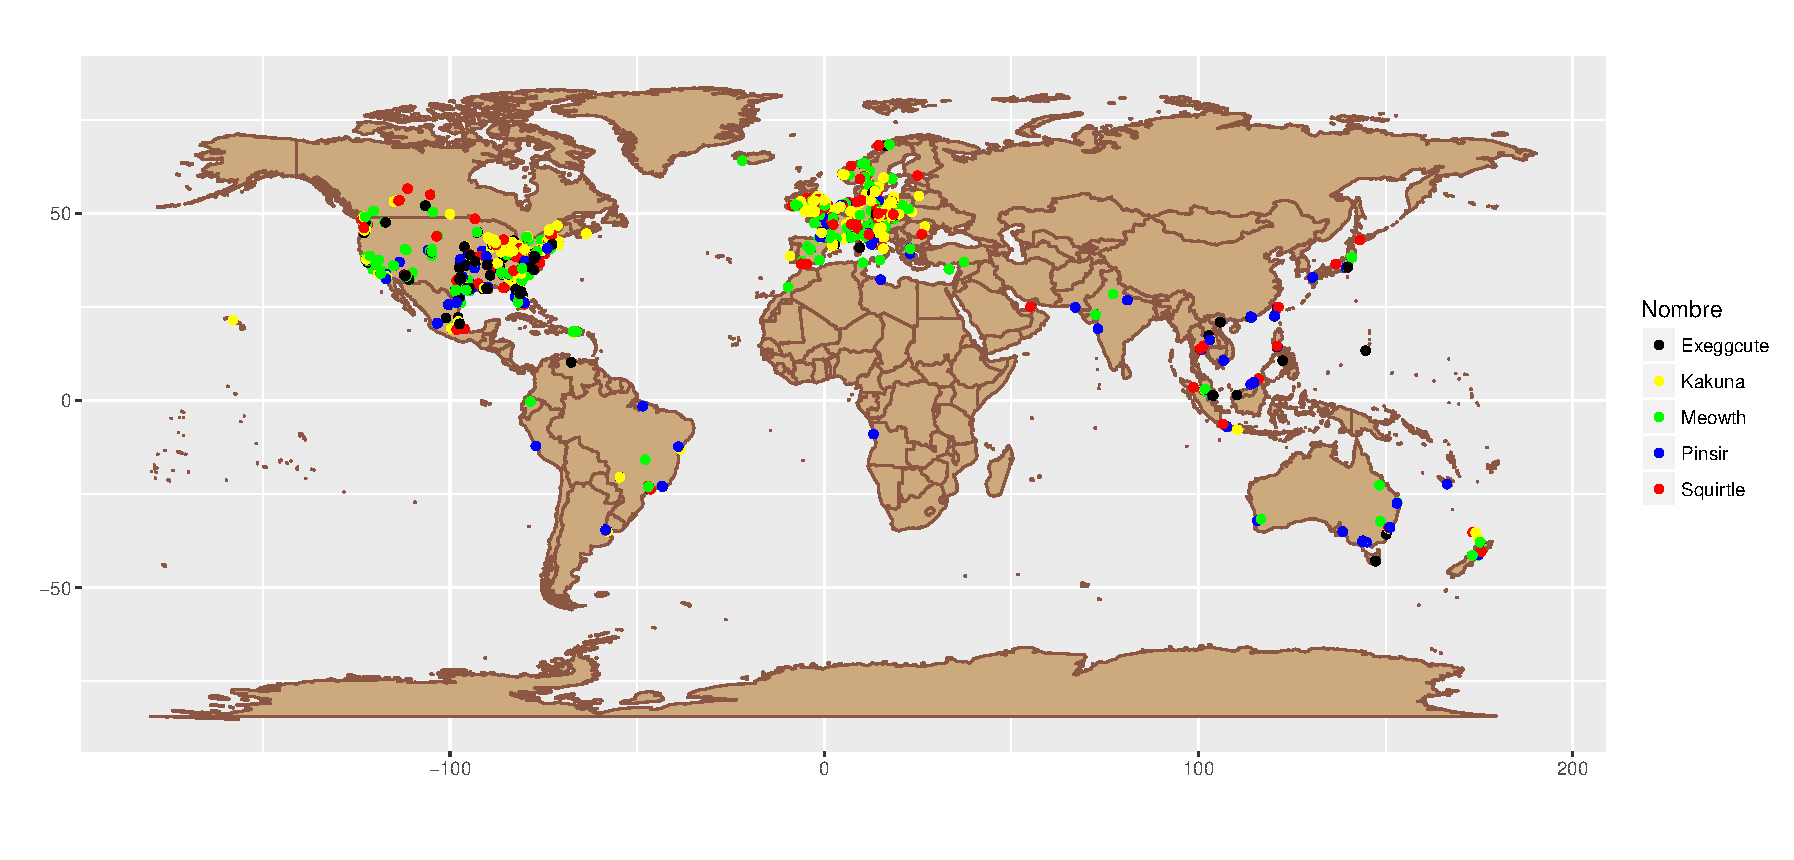
\includegraphics[width = \textwidth]{img/mapaFiltrado.pdf}

Aquí hemos mostrado los avistamiento de las 5 especies de pokemon escogidas. Hemos querido visualizar esto ya que como vimos random forest le daba mucha importancia a los atributos de latitud y longitud. Como podemos observar las 5 especies de pokemon escogidas están muy entremezcladas en el mapa, no pudiendo definir una región clara en la que sólo aparezca un tipo de especie.\\

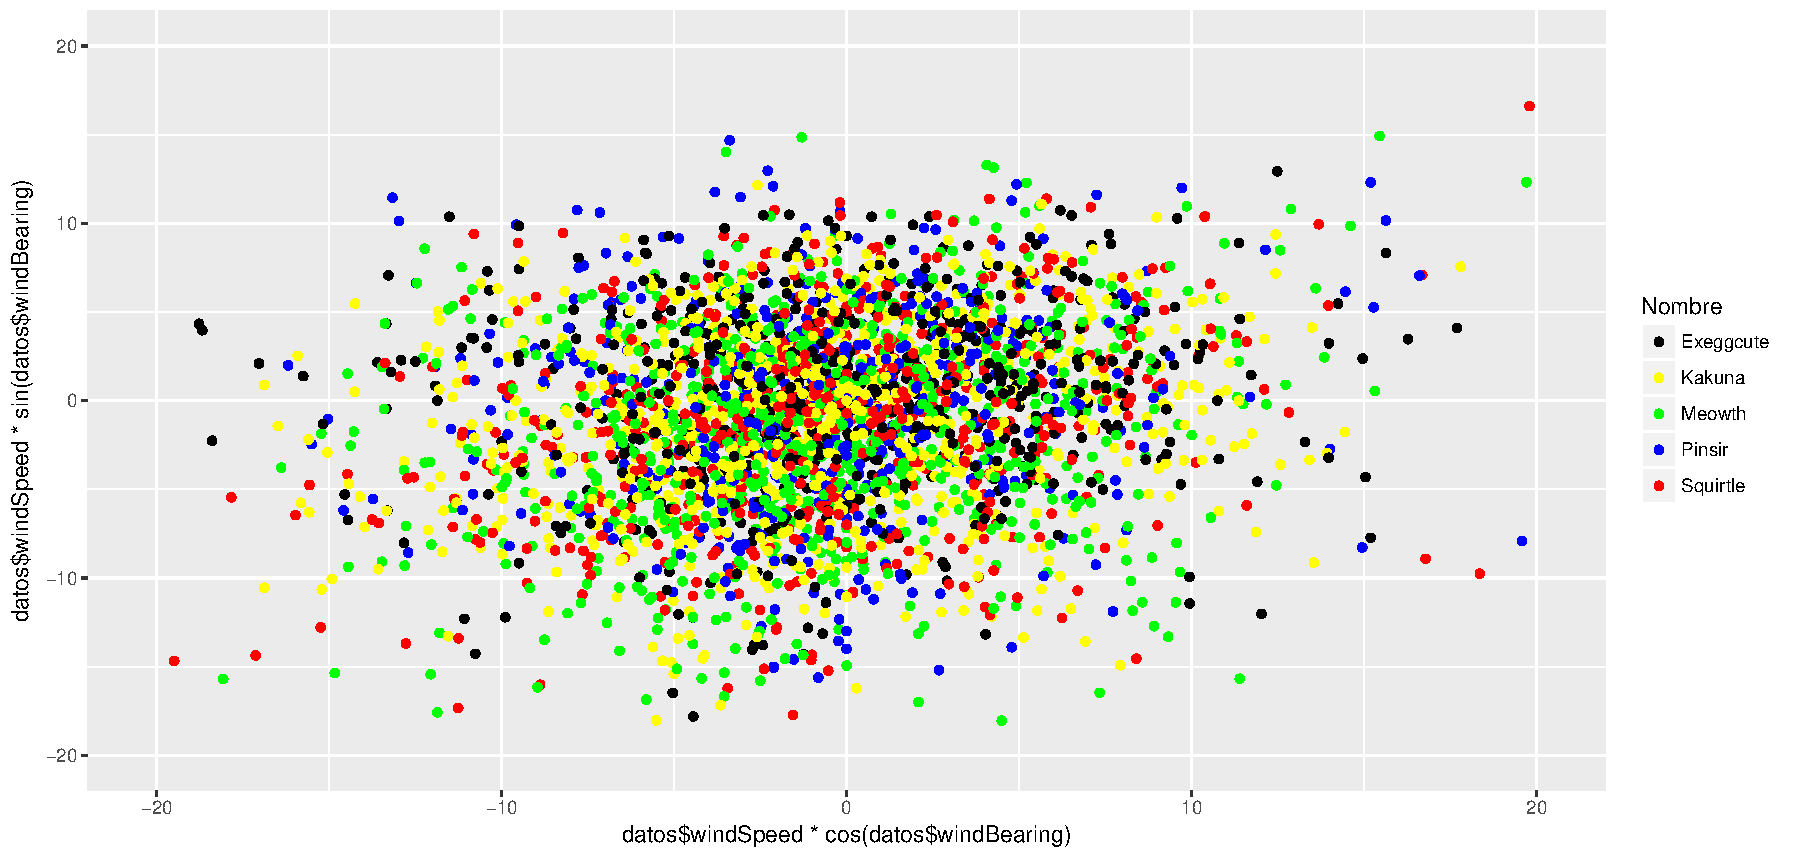
\includegraphics[width = \textwidth]{img/vientoFiltrado.pdf}

Al igual que hicimos para el dataset original hemos querido ver si había algún patrón en la velocidad y dirección del viento para cada una de las especies escogidas, como vemos los resultados han sido similares a los anteriores.

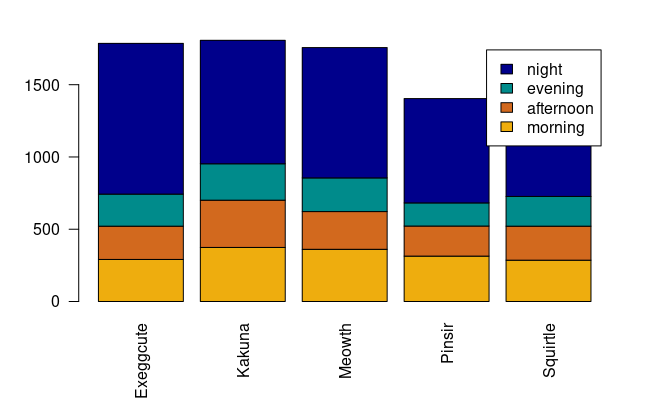
\includegraphics[width = \textwidth]{img/parteDiaFiltrado.png}

Por último aquí vemos, al igual que sucedía con los distintos tipos de pokemon, cómo los avistamientos de las distintas especies se distribuyen a lo largo de todo el día y no se concentran en una sólo parte del día. Con lo cual, a la luz de estas gráficas, no parece que decir que los avistamiento de pokemon tiene una componente aleatoria (al menos para las especies escogidas para hacer clasificación) sea una afirmación incorrecta.